\section{Implementation}
The development of the web interface is made in a local machine using MAMP ( MAC Apache MySQL PHP), and transfer later on to a web server on the university network. 

\subsection{Web server set up - Theis Christensen}
The approach used to implement a small web server on a Linux environment is described, the web server can be access at the address: http://10.1.18.223, it will be used in the evaluative and testing process

The steps used to install a web server on a machine running the Linux distribution Centos are described bellow:
\begin{itemize}
% Apache Install		
		\item Installing Apache and bring the server up.\\
			Install daemon that is going to handle HTTP requests on port 80. ( Apache )
			\begin{lstlisting}[language=c, stepnumber=0, tabsize=1]
				# yum install httpd
			\end{lstlisting}
			Start Apache as background process.
			\begin{lstlisting}[language=c, stepnumber=0, tabsize=1]
				# /etc/init.d/httpd start
			\end{lstlisting}			
			The server is tested by typing in a web browser the ip address of the web server, if the installation is successful the index page is loaded being on a newly installed system the following page. 
			\begin{figure}[H]
				\begin{centering}
					%\missingfigure{Webserver first page}
					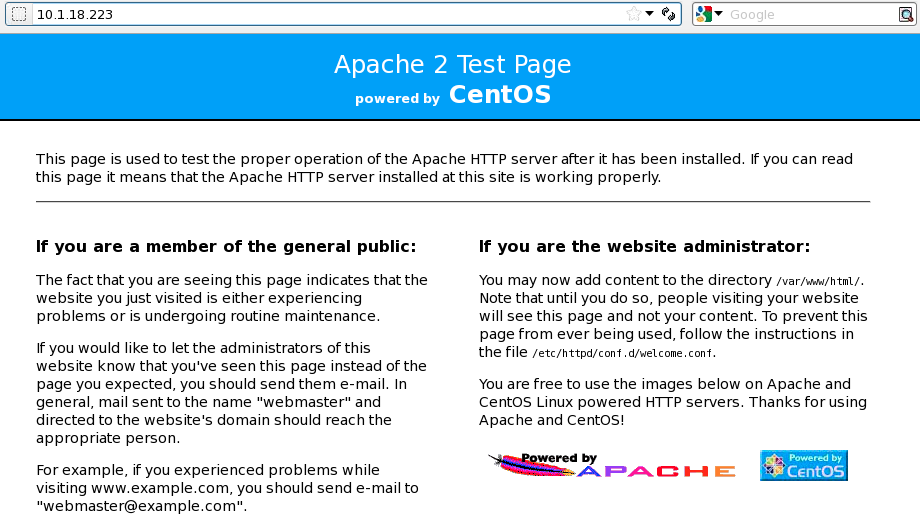
\includegraphics[width=0.8\textwidth]{images/first_web.png}
					\caption{First page apache server running}
				\end{centering}
			\end{figure}
% MySQL Install			
		\item Installing MySQL and bringing the server up\\
			Installing MySQL server and client.
			\begin{lstlisting}[language=c, stepnumber=0, tabsize=1]
				# yum install mysql-server mysql
			\end{lstlisting}
			Start MySQL server as background process.
			\begin{lstlisting}[language=c, stepnumber=0, tabsize=1]
				# /etc/init.d/mysqld start
			\end{lstlisting}
			Testing the MySQL server.
			\begin{lstlisting}[language=c, stepnumber=0, tabsize=1]
				# mysql
			\end{lstlisting}
			Server up and running when the follow response is given.
			\begin{lstlisting}[language=c, stepnumber=0, tabsize=1]
				Welcome to the MySQL monitor.  Commands end with ; or \g.
				Your MySQL connection id is 12
				Server version: 5.0.95 Source distribution

				Copyright (c) 2000, 2011, Oracle and/or its affiliates. All rights reserved.

				Oracle is a registered trademark of Oracle Corporation and/or its
				affiliates. Other names may be trademarks of their respective
				owners.

				Type 'help;' or '\h' for help. Type '\c' to clear the current input statement.

				mysql> 
			\end{lstlisting}
			At this moment the database is set with username root and an empty password. For security reasons a password is set for the MySQL server.\\\\
			Changing MySQL root password
			\begin{lstlisting}[language=c, stepnumber=0, tabsize=1]
				mysql> USE mysql;
				mysql> UPDATE user SET Password=PASSWORD('new password') WHERE user='root';
				mysql> FLUSH PRIVILEGES;
			\end{lstlisting}
			With the instruction \textbf{USE mysql} the database directory mysql is open, and with \textbf{UPDATE user SET Password=PASSWORD ('new password') WHERE user='root'} the password for the user 'root' is updated to the desired one. \textbf{FLUSH PRIVILEGES} erases the privileges in cache and reloads the the new privileges in the MySQL server.
% PHP Install
		\item Installing PHP \\
		Install PHP scripting language and necessary modules for MySQL server integration.
		\begin{lstlisting}[language=c, stepnumber=0, tabsize=1]
			# yum install php php-mysql
		\end{lstlisting}
			php: scripting language compiler\\
			php-mysql: mysql functions to be called from a PHP script\\
		\\
		A file is created and added to the root directory of the web server, this file will retrieve all informations regarding Apache, PHP, MySQL and Modules installed.
		\begin{lstlisting}[language=php, stepnumber=0, tabsize=1]
			<?php
				// Shows the in use PHP configuration file.
				phpinfo();
			?>
		\end{lstlisting}
		Pointing the browser to the address http://10.1.18.223/test.php, will give the following result.
		\begin{figure}[H]
			\begin{centering}
				%\missingfigure{PHP info web page on the browser}
				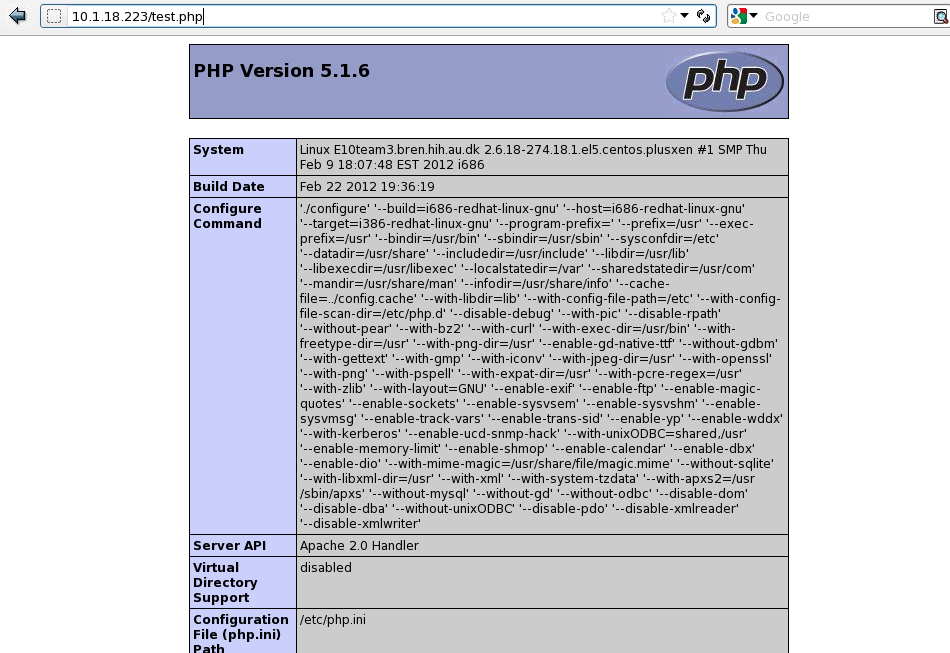
\includegraphics[width=0.8\textwidth]{images/php_info.png}
				\caption{test.php - PHP configuration file}
			\end{centering}
		\end{figure}
% PhpMyAdmin Install
		\item Installing phpMyAdmin\\
		phpMyAdmin is a free web based MySQL database administration environment, without this tool the development of a MySQL database have to be made using the command line, it has become a fundamental tool for most web masters, since the development is faster and fewer errors are made.
		\begin{lstlisting}[language=c, stepnumber=0, tabsize=1]
			# yum install phpmyadmin
		\end{lstlisting}
		The Apache have to be restarted so it can assume the symbolic link to phpMyAdmin tool.
		\begin{lstlisting}[language=c, stepnumber=0, tabsize=1]
			# /etc/init.d/httpd restart
		\end{lstlisting}
		Testing phpMyAdmin by pointing in the web browser to the address http://10.1.18.223/phpmyadmin. The credential used for evaluation purpose are Username: eval Password: ede10eval
		\begin{figure}[H]
			\begin{centering}
				%\missingfigure{PHPmyadmin figure}
				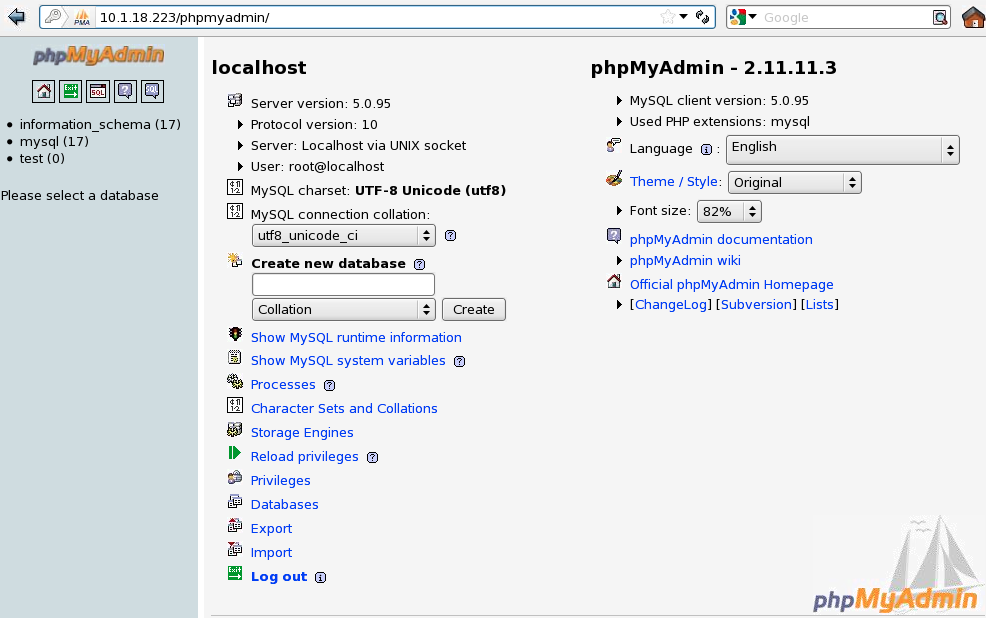
\includegraphics[width=0.8\textwidth]{images/phpmyadmin.png}
				\caption{phpMyAdmin front page}
			\end{centering}
		\end{figure}
\end{itemize}

\subsection{Database - Paulo Fontes}
The tool phpMyAdmin is used to accelerate the process of implementation of the database, the SQL statements generated by the tools is shown in this section and explained in detail.
The database storage engine by default is set to MyISAM, this is changed to InnoDB so foreigner keys and relationships can be used.
To create the tables to store data, a database directory have to be created at first using the statement:
\begin{lstlisting}[language=sql]
		CREATE DATABASE `iEnergy`;
\end{lstlisting}
With the database directory created, the tables can now be created into it. Since the syntax to created the tables is the same, an example table that shows a all possible SQL keywords used in this project is used.
\begin{lstlisting}[language=sql]
		CREATE TABLE IF NOT EXISTS `MEASUREMENTS` (
		  `ID_MEASURE` int(11) NOT NULL auto_increment,
		  `ID_SENSOR` int(11) NOT NULL,
		  `DATE_TIME` datetime NOT NULL,
		  `HUB_PORT` int(11) NOT NULL,
		  `VALUE` float NOT NULL,
		  PRIMARY KEY  (`ID_MEASURE`),
		  FOREIGN KEY (`ID_SENSOR`) REFERENCES `SENSORS` (`ID_SENSOR`)
		  ) ENGINE=InnoDB;
\end{lstlisting}

CREATE TABLE, as the name indicates, is used to create a new table into the database directory. The keywords IF NOT EXIST are add for consistence measures, so the table is not created twice.

To easy identification of the data, all tables have an ID field, this is set as PRIMARY KEY and AUTO\_INCREMENT, it makes sure that new data will have the next ID number and it will be unique. The ID can be as well used to the relationship between tables, in this example the ID\_SENSOR is a foreigner key of the table SENSORS. The ID\_SENSOR is the primary key of the table SENSORS and is related to this table making a constrain in the data to be inserted. When a new data is inserted, the ID\_SENSOR value have to exist in the table sensors, otherwise an error will occur.

At first the name of the field is defined, for example HUB\_PORT will be the name of the field followed by the data type, in this case an integer. The keyword NOT NULL makes impossible to add new data without a defining a value to this field.

The ENGINE keyword defines the storage engine to be used in this table, as explained in the beginning of this section, the use of InnoDB is needed for the relationships and foreigner keys.

%	IMAGE from phpMyAdmin of the structure
%
\begin{figure}[H]
		\begin{centering}
			%\missingfigure{PHPmyadmin figure}
			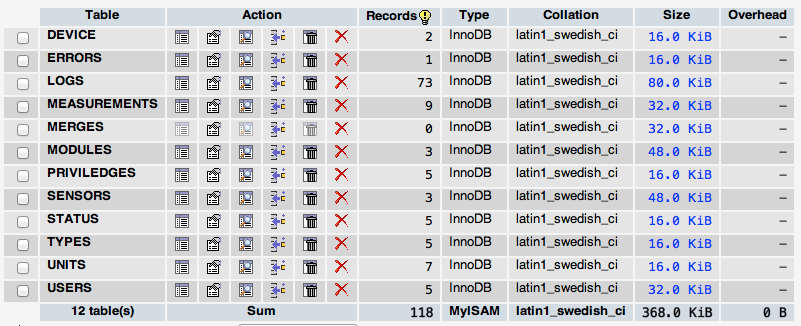
\includegraphics[width=0.8\textwidth]{images/db_struct.png}
			\caption{Database structure and status}
		\end{centering}
\end{figure}


\subsubsection{getData.php} This script is described in this section since is main functionality is to retrieve values from the database using SQL queries and construct a XML file with the data retrieved. Only the Ampere measurements are requested and saved into this database since this is prototype of the system the necessary protocol and structure for the sensors in the modules was not defined.

Script parameters:
\begin{itemize}
	\item unique\_id - this is the only parameter expected by this script, since it will retrieve all the measurements from an unique module/sensor, the URL encoding method for this parameter have to be POST.
\end{itemize}

Several requests to the database are done by this script, each SQL query and is described bellow:

Current power production of the modules:
\begin{lstlisting}[language=sql]
// Current Power Production and Current Power Consuption
	$sql = "SELECT  VALUE FROM `MEASUREMENTS` WHERE `ID_SENSOR`=".$_POST['unique_id']." ORDER BY ID_MEASURE DESC LIMIT 1";
	$res = $con->query($sql);
	$row = $res->fetch_row();
	if($row[0]>0){
		$c_pw_pro = ($row[0]*$voltage)."W ";
		$c_pw_con = "0W ";
	} else if ($row[0]<0){
		$c_pw_con = ($row[0]*$voltage*-1)."W ";
		$c_pw_pro = "0W ";
	} else {
		$c_pw_pro = "0W ";
		$c_pw_con = "0W ";
	}
\end{lstlisting}

The SQL query, uses the keyword \textbf{SELECT} to show the value of the column \textbf{VALUE}, \textbf{FROM} the table \textbf{MEASUREMENTS}, \textbf{WHERE} the field \textbf{ID\_SENSOR} match with the \textbf{unique\_id} send by parameter, the results are \textbf{ORDER BY} the column \textbf{ID\_MEASURE}, from the last inserted value to the first(\textbf{DESC}), with a \textbf{LIMIT} of \textbf{1} result.

The result of this query is the last data entry in the table. If the value is negative it will be multiplied by the voltage and -1, this is the current power consumption. If positive it will be multiplied by the voltage and assigned to the current power production.

Total Power Production:
\begin{lstlisting}
	$sql = 'SELECT SUM(VALUE) 
			FROM `MEASUREMENTS` 
			WHERE `ID_SENSOR`='.$_POST['unique_id'].'
			AND DATE_TIME>(SELECT DATE_TIME FROM LOGS WHERE ID_MODULE='.$_POST['unique_id'].' ORDER BY DATE_TIME DESC LIMIT 1)';
	$res = $con->query($sql);
	$row = $res->fetch_row();
	$tt_pw_pro = ($row[0]*$voltage)."W ";
\end{lstlisting}

The SQL query, uses the keyword \textbf{SELECT} to retrieve the addition (\textbf{SUM}) of the values from the column \textbf{VALUE}, \textbf{FROM} the table \textbf{MEASUREMENTS}, \textbf{WHERE} the field \textbf{ID\_SENSOR} match with the \textbf{unique\_id} send by parameter, AND the columns DATE\_TIME is greater than the result from the  \textbf{SELECT} value of the field \textbf{DATE\_TIME FROM} table LOGS \textbf{WHERE} the \textbf{ID\_SENSOR} match with the \textbf{unique\_id} send by parameter, this result is \textbf{ORDER BY} the column \textbf{DATE\_TIME}, from the last inserted value to the first(\textbf{DESC}), with a \textbf{LIMIT} of \textbf{1} result.

This query returns the addition of all data in column VALUE from the table measurements after the date and time of the last log entry. This way the total power production seen in the user interface corresponds to the uptime of the module/sensor.

Average power production:
\begin{lstlisting}[language=sql]
	// Average Power Production
	$sql = 'SELECT AVG(VALUE) 
			FROM `MEASUREMENTS` 
			WHERE `ID_SENSOR`='.$_POST['unique_id'].'
			AND DATE_TIME>(SELECT DATE_TIME FROM LOGS WHERE ID_MODULE='.$_POST['unique_id'].' ORDER BY DATE_TIME DESC LIMIT 1)';
	$res = $con->query($sql);
	$row = $res->fetch_row();
	$avg_pw_pro = ($row[0]*30)."W ";
\end{lstlisting}

This query is similar to the total power production, instead of the addition of the data in the column VALUES the average is made. This will give the average of values since the last data entry in the table logs.

Module status:
\begin{lstlisting}[language=sql]
	// Status
	if($_SESSION['error_device']==1){
		$stat = "Connection Failed";
	} else {
	
	$sql = 'SELECT `STATUS`.NAME, `STATUS`.ID_STATUS
			FROM STATUS 
			INNER JOIN LOGS ON `STATUS`.ID_STATUS = `LOGS`.ID_STATUS
			WHERE `ID_MODULE`='.$_POST['unique_id'].'
			ORDER BY `LOGS`.ID_LOG DESC 
			LIMIT 1';
	
	$res = $con->query($sql);
	$row = $res->fetch_row();
	
	if($row[0]==""){
		$stat = "Disconnected";
		$id_stat = 2;
	} else {
		$stat = ($row[0]);
		$id_stat = $row[1];
	}
	
	if($row[1]!=3){
			$uptime = " --- ";
			$c_pw_pro = " --- ";
			$c_pw_con = " --- ";
			$tt_pw_pro = " --- ";
			$avg_pw_pro = " --- ";
	} ...
\end{lstlisting}

The SQL query, uses the keyword \textbf{SELECT} to show the values of the columns \textbf{NAME} and \textbf{ID\_STATUS}, \textbf{FROM} table \textbf{STATUS}, when joined (\textbf{INNER JOIN ON}) with table \textbf{LOGS} where the \textbf{STATUS.ID\_STATUS} match with \textbf{LOGS.ID\_STATUS}, and \textbf{WHERE} the field \textbf{ID\_MODULE} match with the \textbf{unique\_id} send by parameter, the results are \textbf{ORDER BY} the column \textbf{ID\_LOG}, from the last inserted value to the first(\textbf{DESC}), with a \textbf{LIMIT} of \textbf{1} result.

This query returns the status name and id for the desired module, the returned values are assigned to the variable stat and id\_stat for later use in this script. In case the status id is different then 3, the module will not be running, so no values are shown to the user.

Create the XML result:
\begin{lstlisting}[language=sql]
	echo '<DATA>'.
			 '<C_PW_PRO>'.$c_pw_pro.'</C_PW_PRO>'.
			 '<C_PW_CON>'.$c_pw_con.'</C_PW_CON>'.
			 '<TT_PW_PRO>'.$tt_pw_pro.'</TT_PW_PRO>'.
			 '<AVG_PW_PRO>'.$avg_pw_pro.'</AVG_PW_PRO>'.
			 '<UPTIME>'.$uptime.'</UPTIME>'.
			 '<STAT id_stat="'.$id_stat.'">'.$stat.'</STAT>'.
			 '<M1 id="'.$m_id[1].'" name="'.$m_name[1].'" status="'.$m_status[1].'" id_status="'.$m_id_status[1].'"></M1>'.
			 '<M2 id="'.$m_id[2].'" name="'.$m_name[2].'" status="'.$m_status[2].'" id_status="'.$m_id_status[2].'"></M2>'.
			 '<PRIV>'.$priv.'</PRIV>'.
			 '<DEV_ERROR>'.$_SESSION['error_device'].'</DEV_ERROR>'.
			'</DATA>';
\end{lstlisting}
XML as HTML is a markup language, using elements defined by tags. JavaScript is able to translate XML files with built-in objects, this allows the return of a large amount of data at once, reducing the number of scripting needed and requests to the web server.

The construction of the XML file can be seen above, the main element is DATA, having several 'child nodes'. This nodes (like HTML) can have several attributes, for example the element M1 and M2 contain attributes that defines the modules connected to the port 1 and 2 of the energy hub.

\subsection{Communication - Dennis Madsen}
The communication between the several components of the system is crucial, data is retrieved at a high rate from the modules, so an effective communication between the energy hub and the web server is implemented. Among the communication with the energy hub, the web interface needs a constant connection with the MySQL server, so data can added and retrieved from the database.

\subsubsection{savedata.php}
A background application running in the energy hub converts the measurement sent through PLC (UART) to a HTTP request \textbf{savedata.php?sensor\_id=ID Sensor\&value=Sensor Measurement\&hub\_port=Hub Port}.

Script parameters:
\begin{itemize}
	\item sensor\_id - Id of the sensor to where save data.
	\item value - the vlue to be saved
	\item hub\_port - the connected port of the module
	\item op - status, change status of a module. <unique\_id><new status>, this is added to the log table.
\end{itemize}
\begin{lstlisting}[language=php]
<?php
	function changeStatus($con){
		$date = getdate();
		$today = $date['year'].'-'.$date['mon'].'-'.$date['mday'].' '.$date['hours'].':'.$date['minutes'].':'.$date['seconds'];
		$sql = 'INSERT INTO `LOGS` (
				`ID_LOG` ,
				`ID_MODULE` ,
				`DATE_TIME` ,
				`ID_STATUS` ,
				`ID_USER` ,
				`ID_ERROR` 
				)
				VALUES (
				NULL , \''.$_GET['id_module'].'\', \''.$today.'\', \''.$_GET['id_status'].'\', \''.$_SESSION['id_user'].'\', \'1\'
				)';
		if($con->query($sql)){
			echo "Success";
		}
		$sql = 'UPDATE `MODULES` SET `HUB_PORT` = '.$_GET['hub_port'].' WHERE `MODULES`.`UNIQUE_ID` ='.$_GET['id_module'];
		
		if($con->query($sql)){
			echo "Success";
		}
	}
	
	if(isset($_GET['op'])){
		
		switch ($_GET['op']){
			case "status": changeStatus($con); break;	
		}
		
	} else {
		$date = getdate();

		$today = $date['year'].'-'.$date['mon'].'-'.$date['mday'].' '.$date['hours'].':'.$date['minutes'].':'.$date['seconds'];

		if(isset($_GET['sensor_id']) && isset($_GET['value']) && isset($_GET['hub_port'])){
			$sql= "INSERT INTO `MEASUREMENTS` (".
				  "`ID_MEASURE` ,".
			  	  "`ID_SENSOR` ,".
			  	  "`DATE_TIME` ,".
			  	  "`HUB_PORT` ,".
			  	  "`VALUE`) ".
			  	  "VALUES (NULL , '".$_GET['sensor_id']."', '".$today."', '".$_GET['hub_port']."', '".$_GET['value']."')";
	
			$con->query($sql); // Run the query in the MySQL server
			echo $sql;
		}	else {
			echo 'Invalide parameters';	
		}
	}
	
?>
\end{lstlisting}

This script saves the measurement retrieved from a sensor to the database. At first it established the connection to the MySQL server so SQL requests can be made.
A PHP function returns an array with the current date and time, this is formatted into YYYY-M-D H:M:S, after it can be saved to the MEASUREMENTS table. The script collects all the parameters send through the URL encoding GET, a SQL code is generated and a request made to the MySQL server, the data is added to the MEASUREMENTS table.

In case of status changes, a parameter \textbf{op} is encode with the method GET and if it value is 'status' the function changeStatus() will be called. This function will update the HUB\_PORT on the table MODULES and insert a new log to the table LOGS. The request for this functionality is  \textbf{savedata.php?op=status\&id\_module=MODULE ID\&id\_status=STATUS TO CHANDE TO\&hub\_port=HUB\_PORT}.

\subsubsection{sendcmd.php}

The web interface is able to send commands to the energy hub and the modules using the\\ \textbf{sendcmd.php?id\_module=\textless module id\textgreater\&cmd=\textless command to be send\textgreater }. The id\_module tells the hub which module the command should be send.
No verification is made of the send command by the web server or the energy hub unless the command is specifically send to the hub.

\begin{lstlisting}[language=php]

<?php
	
	// SQL request for the device page.
	require_once("includes/db_connect.php");
	
	if(isset($_GET['cmd']) && isset($_GET['id_module'])){
		
		$device_port = 5555;
			
		$sql= "SELECT IP ". 
			  "FROM `DEVICE` ". 
			  "ORDER BY ID_DEVICE DESC ".
			  "LIMIT 1";
		
		$res = $con->query($sql); // Run the query in the MySQL server
		
		$row = $res->fetch_row();
		
		$device_ip = $row[0];
		
		if (!$socket=socket_create(AF_INET, SOCK_STREAM, SOL_TCP)){
			exit (socket_strerror(socket_last_error()));
		}
	
		if (!socket_connect($socket,$device_ip,$device_port)){
			exit (socket_strerror(socket_last_error()));
		}
	
		$str = $_GET['cmd'].';'.$_GET['id_module'].';'.$_GET['dir'];
		
		socket_write($socket,$str);
	
		$msg='';
		$c='';
    	
		while(socket_recv($socket, $c, 256,0)){
  			if($c != null) {
   				$msg .= $c;
			}
		}
		
		echo $msg;
        
		socket_close($socket);
		
	} else {
		echo 'Command or Module Id not set';
	}

?>
\end{lstlisting}

At first the script will get the ip address of the energy hub, a SQL query retrieves the last IP address added to the table DEVICES. With the energy hub ip and a predefined port, a connection is created using a TCP socket for the communication between the energy hub and the web server. The parameters are collected from the encode URL and translated to a recognized format in the energy hub. The data is send to the energy hub and a answer of success or not is returned.

This script is called in background by a client side script, this will handle how to warning the user in case a problem occurs.

\subsubsection{saveip.php}

This script is called by the background application running on the energy hub, it saves the IP address given by DHCP, this is used for further communication between the web server and the energy hub.
\begin{lstlisting}[language=php]
	require_once("includes/db_connect.php");

	if(isset($_GET['ip'])){
		$sql= "INSERT INTO `DEVICE` (".
			  "`ID_DEVICE` ,".
		  	  "`IP`)".
		  	  "VALUES (NULL , '".$_GET['ip']."')";
	
		$con->query($sql); // Run the query in the MySQL server
		
		// No feedback needed since the energy hub will not expect an answer.
		
	} else {
		echo 'IP not set';
	}
\end{lstlisting}
The ip address is send by the GET method (saveip.php?ip=127.0.0.1), this is how the data in encoded into a URL, being collected in the variable \$\_GET['ip']. 
A \$sql variable string is created containing the SQL code to be run at the MySQL server.

\subsubsection{db\_connect.php}

For the communication to the database a driver is used in PHP that provides an interface to the MySQL server. The PHP mysqli extension (MySQL improved) is used in this project, this is recommend for MySQL servers version 4.1.3 or later. This extension provides several benefits as a objective-oriented interface, support for multiple statements, embedded server support and more can be found in the MySQL documentation.

\begin{lstlisting}[language=php]
	require_once("db_globals.php");
	
	$con = new mysqli(DB_HOST,DB_USER,DB_PASS,DB_NAME); // Creates new mysql connection
	
	if($con->connect_error){
		echo "Failed to connect to MySQL: (" . $con->connect_errno . " ) ". $con->connect_error;
	} 
	else { echo "Connection established"; }
\end{lstlisting}

In this script an object is instantiated with a connection to the MySQL server.

\textit{\$con = new mysqli\textless parameters \textgreater)}

The parameters are included from the db\_globals.php, setting the server host, user, password and database to be used.

\subsubsection{db\_globals.php}

Using a script to define the parameters for the MySQL connection, 
All the scripts that need to use the global parameters for the connection to the MySQL server, should include db\_globals.php as shown in the db\_connect.php above.

\begin{lstlisting}[language=php]
	// MySQL condifuration
	DEFINE ('DB_USER','root');
	DEFINE ('DB_PASS','pass');
	DEFINE ('DB_HOST','localhost');
	DEFINE ('DB_NAME','iEnergy');
\end{lstlisting}

The global parameters the connection to the MySQL server are define in this script.

\begin{itemize}
	\item DB\_USER - Database user name with read, write and execute permissions.
	\item DB\_PASS - Password for the user
	\item DB\_HOST - Hostname for the MySQL server, if running at the same host as the PHP server, localhost or 127.0.0.1 should be used.
	\item DB\_NAME - Database name to connect to.
\end{itemize}

\subsection{Login - Theis Christensen}

The login script is called in background by the client side script popUp, this handles the login and logout of the users to the system. Both client and server side scripts for the login functionality is explained in this section.

\subsubsection{login.php}The server side script login, receives the credentials given by the user and compares with the ones stored in the database. In case of match, the privilege ID is retrieved and a user session is created with the user name and privilege id. In case of logout the session privilege is set to 0 and a message is returned to the client side script to handle.
\begin{lstlisting}[language=php]
	if (isset($_POST['logout'])){ // If logout is set by PORT encoded URL request
		
		echo "logout";			  // Return logout for the javascript
		$_SESSION['priv']=0;	  // Set the priv to 0
		
	} else if(isset($_POST['user']) && isset($_POST['pass'])){
		
		$sql = "SELECT ID_PRIV WHERE NAME='".$_POST['user']."'AND PASS='".$_POST['pass']."'"; // SQL statment contruction (No encryption in password)
		
		$res = $con->query($sql); // MySQL request

		if ($res->num_rows==1){ // See if any value is returned, if true assign privelege to session priv.
			
			$row = $res->fetch_row();	
			$_SESSION['priv']=$row[0];
			echo "ok";
		} else {
			echo "Wrong credentials";
		}
	}
\end{lstlisting}

Passwords are not encrypted in the table USERS since no user management web application was developed, the user names and passwords have to be inserted 'manually' into the database using phpMyAdmin. This system doesn't require high level of security since it cannot be accessible form the outside the university network.

\subsubsection{popUp.js}
The popUp script, handle the login actions to the web interface. When the locker is clicked, the window is blocked with a dark grey background and the credentials are asked from the user. The user is able to cancel this action, or input the credential to login into the web interface administration. When the user name and password are inserted and the ok button clicked, a background request is made to the script login.php. This will return an 'ok' if the credentials are correct, or an error message to be shown to the user if no match is found on the table USERS. The implementation of the login.php script is explained earlier in this project.

Function sendCred, sends a background request to the server, returns ok if success and error message otherwise. 

Parameters:
\begin{itemize}
	\item type - 0 for logout, 1 for login
	\item str - path for the login.php script, normal path to this script would be the root directory of the server, in this way customized login scripts can be used.
\end{itemize}

%	IMAGE from login popup
\begin{figure}[H]
		\begin{centering}
			%\missingfigure{PHPmyadmin figure}
			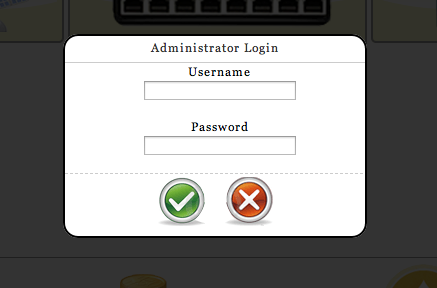
\includegraphics[width=0.6\textwidth]{images/login.png}
			\caption{Login window}
		\end{centering}
\end{figure}

\subsection{Error Handling - Paulo Fontes}
The implementation of an error handling will keep the web interface more reliable, improve user experience and alert the administrators to a error situation. A error handling PHP script is called in background, this script will test the communication between the web server and the energy hub, and the communication to the MySQL server. As described in the analysis in this report, the user interface is blocked giving the message warning when the communication with the MySQL server is lost and a warning is given to the user when no communication with energy hub is found.

\subsubsection{errorhandler.php} The error handler PHP script is included in each web page before any other script, this script is included when a page is loaded and is recursively called in background to test the connections. The script gives a XML response, when called as background so the client side JavaScript can handle the real time warnings to the user. This method can be called as active error handle, since it acts in real time, usually error handling is implemented when is need to do some action, for example retrieve data from database. With this system the user is immediately blocked from doing any action until the situation is solved.

Since this script is included before everything else, the HTML, JavaScript and CSS layout is included in the file. Bellow several code blocks were extracted for and easier explanation, the full code can be seen using the application SeeIt and in the appendix of this report.

At first and most important the database connection have to be tested, as such a connection to the database is attempted. If the connection is successful the database error session variable will be 0. In case of connection failure the error variable will be changed to one and kept until the connection is re established, changing the session error variable to 2. This will tell the client side script that the situation was solved and in the next test the variable is changed to 0 again. This can be seen in the code bellow.
\begin{lstlisting}[language=php]
	
	if ($_SESSION['error_db']>1) { 
		$_SESSION['error_db']=0;
	}

	$_SESSION['error_device']=0;

	// Test DB connection
	require_once("includes/db_globals.php");
	
	$con = mysql_connect(DB_HOST,DB_USER,DB_PASS,DB_NAME);
	
	if(!$con){
		$_SESSION['error_db']=1;
		$error = "Failed to connect to database: ". mysql_error();
	} else {
		if ($_SESSION['error_db']==1){
			$_SESSION['error_db']=2;
		} else {
			$_SESSION['error_db']=0;	
		}
	}
\end{lstlisting}

If no error regarding the database connection is acknowledge, the ip address for the energy hub is retrieved and the connection with the energy hub can be established.

\begin{lstlisting}[language=php]
if($_SESSION['error_db']==0){
		
		$device_port = 5555;
		
		$con = new mysqli(DB_HOST,DB_USER,DB_PASS,DB_NAME);
		
		$sql= "SELECT IP ". 
			  "FROM `DEVICE` ". 
			  "ORDER BY ID_DEVICE DESC ".
			  "LIMIT 1";
		
		$res = $con->query($sql);
		
		$row = $res->fetch_row();
		
		$device_ip = $row[0];
\end{lstlisting}

The SQL statement  \textbf{SELECT IP FROM `DEVICE` ORDER BY ID\_DEVICE DESC LIMIT 1} retrieves the last ip address insert in the table. The keywords ORDER BY ID\_DEVICE DESC will show the last data added and the keyword LIMIT 1, limits the number of values return to only one. The value is then fetched from the result and assigned to the variable device\_ip for later use in the connection.

For the communication to the energy hub a socket have to be created and a connection established. In case of one of this steps don't work (Socket creation and Connection), a error session variable is set to 1, the client side application will catch this error and alert the user for such situation. The socket is closed after testing to leave the connection path open for new tests or commands to be send.

\begin{lstlisting}[language=php]
		if (!$socket=socket_create(AF_INET, SOCK_STREAM, SOL_TCP)){
			$_SESSION['error_device']=1;
		} else {
			$_SESSION['error_device']=0;
		}
	
		if (!socket_connect($socket,$device_ip,$device_port)){
			$_SESSION['error_device']=1;
		} else {
			$_SESSION['error_device']=0;
		}
		
		socket_write($socket,"a");
		
		socket_close($socket);
	
	}
\end{lstlisting}

The error handle client side (JavaScript) and server side (PHP) are developed at the same time, since the cooperation between both is essential for the proper operation of the error handling system.

This block of code is used only by the client side script, it make a request to the errorhandle.php with the encoded URL variable op=d, this block will return an XML response. The client side script then interpret the answer and reacts according to the errors.
\begin{lstlisting}[language=php]
	if(isset($_GET['op']) && $_GET['op']=='d'){
		
		echo '<ERROR>'.
			    '<DB>'.$_SESSION['error_db'].'</DB>'.
				'<DEVICE>'.$_SESSION['error_device'].'</DEVICE>'.
			  '</ERROR>';
		
	} else {
\end{lstlisting}

The else statement in this code indicates that, if the script was not called by the error.js, then it will include the necessary HTML, CSS and JavaScript to the file where it was included.

An example of this situation is found at the index.php, the first lines of this script starts the session and includes errorhandle.php.

\begin{lstlisting}[language=php]
<?php
	session_start();
	
	require_once("errorhandler.php");
	
	require_once("includes/db_connect.php");
?>
\end{lstlisting}

\subsubsection{error.js}
This script catches and handle errors in the client side, it uses background requests to the PHP script errorhadle.php. By the XML response it acts according the situation. JavaScript is a dynamic language with a lot of potential, and this is used in detail in this script.Meaningful blocks will be extracted from the code and explained here.

Three functions are part of this script, being two of them for animation to improve the user experience, they are not documented in this section. The remaining function is the mains focus of the error handling system, is called makeTests().

This functions initialize the variables req for the URL request, db\_error and dev\_error that will be assigned with the values returned by the request.
At first the browser is tested to define which HTTP request object to use, the main difference is between IE (version 5 and 6) form Microsoft and the rest ot the browsers, since IE (version 5 and 6) uses an ActiveX object to deal with background requests.
\begin{lstlisting}[language=php]
	var req;
	var db_error;
	var dev_error;
	
	if(window.XMLHttpRequest){
		req	= new XMLHttpRequest();
	} else {
		req = ActiveXObject("Microsoft.XMLHTTP");	
	}
\end{lstlisting}

The open and send methods from the XMLHttpRequest object, are used to send a request to the server. The 'open' method specifies the type of encoding used in the URL (GET or POST) and if the request is synchronous or not. The 'send' method sends the request to the server, parameters are needed in case of POST encoding method. 

\begin{lstlisting}[language=php]
	req.open("GET","/errorhandler.php?op=d",false);
	req.overrideMimeType('text/xml');
	req.send();
	
	var result = req.responseXML;
\end{lstlisting}

The result variable is initialized and the returned XML data is assigned to it, this data is then extracted and used according to the situation. An example of retrieved XML data can be seen bellow:

\begin{lstlisting}[language=xml]
		<ERROR>
			<DB>0</DB>
			<DEVICE>0</DEVICE>
		</ERROR>
\end{lstlisting}

%	IMAGE from ERROR HANDLING database and device
%

Graphical representation of an error in the connection to the database and communication to the energy hub device.
\begin{figure}[H]
	\begin{tabular}{ c c }
		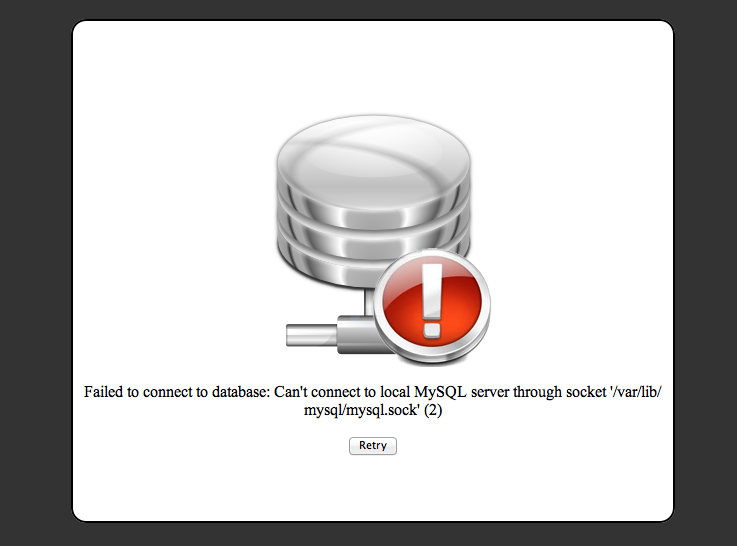
\includegraphics[width=0.5\textwidth]{images/error_db.png}
&
		
\includegraphics[width=0.2\textwidth]{images/error_device.png}
\end{tabular}
\caption{Database Error and Device communication Error}
\end{figure} 

\subsection{User Experience - Dennis Madsen}
The user experience is improved by the client side scripts, HTTP requests are make as background using AJAX methods. This method is used in all the client side scripts in this system. The diagram above describe this method.

How AJAX Works:

\begin{figure}[H]
	\begin{centering}
		%\missingfigure{Webserver first page}
		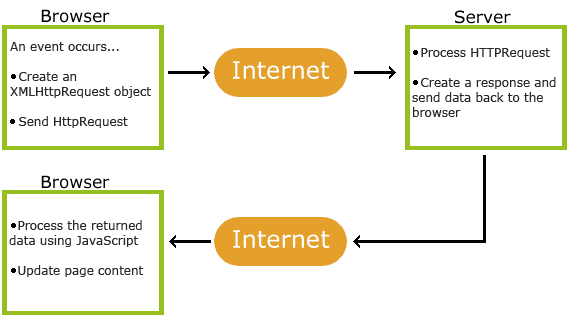
\includegraphics[width=0.5\textwidth]{images/ajax.png}
		\caption{http://www.w3schools.com/ajax/ajax\_intro.asp}
	\end{centering}
\end{figure}

JavaScript is used to handle the returned values and change the layout according to them, this add great functionalities in user experience, since just parts of the page are dynamical changed with now need for refreshing the page with every action.

\subsubsection{control.js}
This script update the data displayed to the user without the need of refreshing the all page. It controls all the dynamics of the page such as send commands to the energy hub, get data from the database and displaying it to the users. The code for this script is extensive since it is the controller of the client side interface, as such the code can be seen in appendix or with the application SeeIt.

The script con\_control.js in the root directory, is a striped down version of the control script, since its only functionality is to show the modules connected to the energy hub in the main page.

Function getData, makes a background request to the server, returning an XML file. This file is then handle and the correspondent fields on the user interface are updated. (See appendix for code)

Parameters:
\begin{itemize}
	\item id - module id to retrieve stored values form the database.
	\item str - path for the getdata.php script, normal path to this script would be the modules/ directory in the server structure, this method allows the modules to use a different script.
\end{itemize}

Function sendCmd, send a background request to the server, returning the success or not of the command. The result is handle and the user is notified if the command was not successful. 

Parameters:
\begin{itemize}
	\item module\_id - ID of the module to who the energy hub is going to transmit the command.
	\item cmd - command to be send to the module/energy hub.
\end{itemize}